\documentclass[12pt,a4paper]{article}

% ─── Page Layout ───────────────────────────────────────────────────────────────
\usepackage[a4paper, margin=0.8in, headheight=14pt]{geometry}

% ─── Fonts (XeLaTeX) ───────────────────────────────────────────────────────────
\usepackage{fontspec}
\usepackage{unicode-math}
\setmainfont{TeX Gyre Pagella}
\setmonofont[Scale=0.88]{TeX Gyre Cursor}
\setmathfont{Latin Modern Math}

% ─── Packages ──────────────────────────────────────────────────────────────────
\usepackage{xcolor}
\usepackage{colortbl}
\usepackage{titlesec}
\usepackage{enumitem}
\usepackage{tabularx}
\usepackage{booktabs}
\usepackage{array}
\usepackage{amsmath}
\usepackage{tikz}
\usetikzlibrary{shapes.geometric, arrows.meta, positioning, calc, fit, decorations.pathreplacing}
\usepackage{tcolorbox}
\tcbuselibrary{skins, breakable}
\usepackage{hyperref}
\usepackage{fancyhdr}
\usepackage{graphicx}
\usepackage{microtype}
\hyphenpenalty=10000
\exhyphenpenalty=10000
\sloppy
\usepackage{caption}
\usepackage{setspace}
\usepackage{multirow}
\usepackage{tocloft}

% ─── Q&A helper ────────────────────────────────────────────────────────────────
\newcommand{\Q}[1]{\textbf{#1}\par\noindent\ignorespaces}

% ─── Colour Palette ────────────────────────────────────────────────────────────
\definecolor{myred}{RGB}{196,30,58}
\definecolor{mydark}{RGB}{30,30,50}
\definecolor{mygreen}{RGB}{14,120,80}
\definecolor{myteal}{RGB}{0,130,140}
\definecolor{myamber}{RGB}{180,100,0}
\definecolor{mypurple}{RGB}{100,30,160}
\definecolor{mygray}{RGB}{246,247,249}
\definecolor{mgframe}{RGB}{180,185,200}
\definecolor{watermark}{RGB}{145,150,170}
\definecolor{hdrred}{RGB}{250,232,235}
\definecolor{hdrgreen}{RGB}{220,244,233}
\definecolor{hdrteal}{RGB}{220,242,244}
\definecolor{hdramber}{RGB}{253,242,215}
\definecolor{hdrpurple}{RGB}{238,228,255}
\definecolor{hdrgray}{RGB}{238,240,245}
\definecolor{rowalt}{RGB}{250,251,253}

% ─── Section Formatting ────────────────────────────────────────────────────────
\titleformat{\section}
  {\large\bfseries\color{myred}}{\thesection.}{0.5em}{}
  [\vspace{1pt}{\color{myred}\rule{\linewidth}{0.8pt}}]
\titleformat{\subsection}
  {\normalsize\bfseries\color{myteal}}{\thesubsection}{0.5em}{}
\titlespacing*{\section}{0pt}{18pt}{7pt}
\titlespacing*{\subsection}{0pt}{11pt}{4pt}

% ─── Paragraph ─────────────────────────────────────────────────────────────────
\setlength{\parindent}{0pt}
\setlength{\parskip}{4pt}

% ─── TOC Styling ───────────────────────────────────────────────────────────────
\renewcommand{\cfttoctitlefont}{\large\bfseries\color{myred}}
\renewcommand{\cftaftertoctitle}{\par\noindent{\color{myred}\rule{\linewidth}{0.8pt}}}
\setlength{\cftbeforetoctitleskip}{0pt}
\setlength{\cftaftertoctitleskip}{6pt}
\renewcommand{\cftsecfont}{\normalsize\bfseries\color{mydark}}
\renewcommand{\cftsecpagefont}{\normalsize\bfseries\color{mydark}}
\renewcommand{\cftsecleader}{\cftdotfill{\cftdotsep}}
\setlength{\cftbeforesecskip}{7pt}
\renewcommand{\cftsubsecfont}{\small\color{mydark}}
\renewcommand{\cftsubsecpagefont}{\small\color{mydark}}
\setlength{\cftbeforesubsecskip}{3pt}
\setlength{\cftsubsecindent}{1.4em}

% ─── Table helpers ─────────────────────────────────────────────────────────────
\renewcommand{\arraystretch}{1.45}
\setlength{\tabcolsep}{6pt}
\arrayrulecolor{mydark}
\newcolumntype{B}[1]{>{\small\bfseries\raggedright\arraybackslash}m{#1}}
\newcolumntype{Y}{>{\small\raggedright\arraybackslash}X}
\renewcommand{\tabularxcolumn}[1]{m{#1}}

% ─── Header / Footer ───────────────────────────────────────────────────────────
\pagestyle{fancy}
\fancyhf{}
\fancyhead[L]{\small\color{myred}\textbf{PE-EC703A}\;\color{mydark}--- Embedded System}
\fancyhead[R]{\small\color{myteal}\textbf{Module 2 Notes}}
\fancyfoot[C]{\small\color{mydark}\thepage}
\fancyfoot[R]{\small\color{watermark}\textit{\copyright\ Biraj}}
\renewcommand{\headrulewidth}{0.5pt}
\renewcommand{\footrulewidth}{0.3pt}

% ─── Hyperref ──────────────────────────────────────────────────────────────────
\hypersetup{
  colorlinks=true, linkcolor=myteal, urlcolor=myteal,
  pdfauthor={Biraj Sarkar},
  pdftitle={PE-EC703A --- Module 2 Notes}
}

% ─── tcolorbox styles ──────────────────────────────────────────────────────────
\tcbset{
  tikzbox/.style={
    colback=mygray, colframe=mgframe, boxrule=0.6pt, arc=4pt,
    left=8pt, right=8pt, top=6pt, bottom=6pt,
    colbacktitle=mgframe, coltitle=mydark,
    fonttitle=\small\bfseries
  },
  defbox/.style={
    colback=hdrgreen, colframe=mygreen, boxrule=0.8pt, arc=4pt,
    left=9pt, right=9pt, top=6pt, bottom=6pt,
    colbacktitle=mygreen, coltitle=white,
    fonttitle=\small\bfseries
  },
  formulabox/.style={
    colback=hdrteal, colframe=myteal, boxrule=0.8pt, arc=4pt,
    left=9pt, right=9pt, top=7pt, bottom=7pt,
    colbacktitle=myteal, coltitle=white,
    fonttitle=\small\bfseries
  },
  examplebox/.style={
    colback=hdramber, colframe=myamber, boxrule=0.8pt, arc=4pt,
    left=9pt, right=9pt, top=6pt, bottom=6pt,
    colbacktitle=myamber, coltitle=white,
    fonttitle=\small\bfseries
  },
  masonbox/.style={
    colback=hdrpurple, colframe=mypurple, boxrule=0.8pt, arc=4pt,
    left=9pt, right=9pt, top=6pt, bottom=6pt,
    colbacktitle=mypurple, coltitle=white,
    fonttitle=\small\bfseries
  },
  exambox/.style={
    colback=hdrpurple, colframe=mypurple, boxrule=1pt, arc=5pt,
    left=10pt, right=10pt, top=8pt, bottom=8pt,
    colbacktitle=mypurple, coltitle=white,
    fonttitle=\bfseries,
    breakable, title after break={\textbf{Frequently Asked / Viva Questions (contd.)}}}
}
\tcbset{breakable}

% ─── TikZ styles ───────────────────────────────────────────────────────────────
\tikzset{
  block/.style={rectangle, draw=myteal, fill=hdrteal,
    text width=2.4cm, align=center, minimum height=0.95cm,
    font=\small, rounded corners=3pt, line width=0.7pt},
  redblock/.style={rectangle, draw=myred, fill=hdrred,
    text width=2.4cm, align=center, minimum height=0.95cm,
    font=\small, rounded corners=3pt, line width=0.7pt},
  netnode/.style={rectangle, draw=myteal, fill=hdrteal,
    text width=1.5cm, align=center, minimum height=0.8cm,
    font=\small, rounded corners=3pt, line width=0.7pt},
  sumjunc/.style={circle, draw=myamber, fill=hdramber,
    minimum size=0.62cm, font=\small, line width=0.8pt},
  snode/.style={circle, draw=mypurple, fill=hdrpurple,
    minimum size=0.55cm, font=\footnotesize, line width=0.7pt},
  arrow/.style={-Stealth, thick, color=mydark},
  redarrow/.style={-Stealth, thick, color=myred},
  line/.style={thick, color=mydark}
}

% ═══════════════════════════════════════════════════════════════════════════════
\begin{document}
% ═══════════════════════════════════════════════════════════════════════════════

\begin{center}
  {\LARGE\bfseries\color{myred} PE-EC703A --- Embedded System}\\[5pt]
  {\normalsize\color{mydark} Semester VII \quad$\bullet$\quad 3L:0T:0P \quad$\bullet$\quad 3 Credits}\\[3pt]
  {\normalsize\color{myteal}\textbf{Module 2 Exam Notes: Embedded Hardware --- Processor \& Memory}}\\[3pt]
  {\small\color{mydark} CGEC \;$|$\; B.Tech ECE (2023--27) \;$|$\; \textit{Biraj Sarkar}}
\end{center}
\vspace{2pt}
\noindent{\color{myred}\rule{\linewidth}{1.5pt}}
\vspace{2pt}

\hypersetup{linkcolor=mydark}
\tableofcontents
\hypersetup{linkcolor=myteal}
\newpage

% ===============================================================================
\section{8051 Microcontroller --- Architecture Overview}
% ===============================================================================

The Intel 8051 is an 8-bit microcontroller introduced in 1980. It is one of the most widely taught architectures in embedded systems education due to its simplicity and self-contained design.

\begin{tcolorbox}[defbox, title={\textbf{8051 Microcontroller}}]
The \textbf{8051} is an 8-bit, single-chip microcontroller with on-chip program memory (ROM), data memory (RAM), I/O ports, timers, a serial port, and interrupt logic. It operates on a Harvard architecture (separate program and data memory buses).
\end{tcolorbox}

\subsection{Key Features of 8051}
\begin{itemize}[leftmargin=*, itemsep=3pt]
  \item \textbf{CPU:} 8-bit ALU, accumulator (A), B register, PSW (Program Status Word).
  \item \textbf{ROM (Program Memory):} 4 KB on-chip; expandable to 64 KB externally.
  \item \textbf{RAM (Data Memory):} 128 bytes on-chip; upper 128 bytes are SFRs (Special Function Registers).
  \item \textbf{I/O Ports:} Four 8-bit bidirectional I/O ports (P0, P1, P2, P3).
  \item \textbf{Timers:} Two 16-bit timers/counters (Timer 0 and Timer 1).
  \item \textbf{Serial Port (UART):} Full-duplex serial communication (TXD/RXD on P3).
  \item \textbf{Interrupts:} Five interrupt sources --- INT0, INT1, Timer0, Timer1, Serial.
  \item \textbf{Clock:} Typically 12 MHz crystal; one machine cycle = 12 clock cycles.
\end{itemize}

\begin{tcolorbox}[tikzbox, title={8051 Internal Architecture Block Diagram}]
\centering
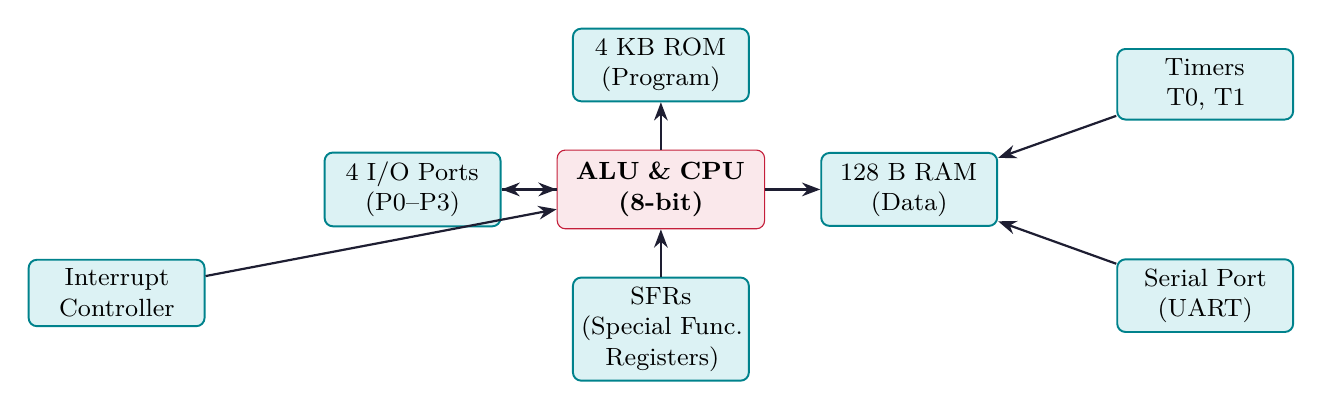
\begin{tikzpicture}[node distance=0.3cm and 0.5cm,
  sblock/.style={rectangle, draw=myteal, fill=hdrteal, text width=2.0cm,
    align=center, minimum height=0.8cm, font=\small, rounded corners=3pt, line width=0.7pt}]
  \node[rectangle, draw=myred, fill=hdrred, text width=2.4cm, align=center,
    minimum height=1.0cm, font=\small\bfseries, rounded corners=3pt] (alu) {ALU \& CPU\\(8-bit)};
  \node[sblock, above=0.6cm of alu] (rom) {4 KB ROM\\(Program)};
  \node[sblock, right=0.7cm of alu] (ram) {128 B RAM\\(Data)};
  \node[sblock, below=0.6cm of alu] (sfr) {SFRs\\(Special Func.\\Registers)};
  \node[sblock, left=0.7cm of alu] (io) {4 I/O Ports\\(P0--P3)};
  \node[sblock, above right=0.4cm and 1.5cm of ram] (tmr) {Timers\\T0, T1};
  \node[sblock, below right=0.4cm and 1.5cm of ram] (ser) {Serial Port\\(UART)};
  \node[sblock, below left=0.4cm and 1.5cm of io] (intr) {Interrupt\\Controller};

  \draw[arrow] (alu) -- (rom);
  \draw[arrow] (alu) -- (ram);
  \draw[arrow] (sfr) -- (alu);
  \draw[arrow] (io) -- (alu);
  \draw[arrow] (alu) -- (io);
  \draw[arrow] (tmr) -- (ram);
  \draw[arrow] (ser) -- (ram);
  \draw[arrow] (intr) -- (alu);
\end{tikzpicture}
\end{tcolorbox}

\subsection{Real-World Interfacing of 8051}
\begin{itemize}[leftmargin=*, itemsep=3pt]
  \item \textbf{LED / Switch:} GPIO pins directly drive LEDs (with current-limiting resistors); switches pulled up to VCC.
  \item \textbf{LCD (16x2):} Driven via P2 (data bus) and P3 control lines (RS, RW, EN).
  \item \textbf{ADC (e.g., ADC0804):} External ADC connected via parallel data bus and control signals.
  \item \textbf{Stepper Motor:} Driven via ULN2003 driver IC connected to P1.
  \item \textbf{Serial Communication:} TXD (P3.1) and RXD (P3.0) connect to MAX232 (RS-232 level converter) for PC communication.
\end{itemize}

% ===============================================================================
\section{ARM Processor Architecture}
% ===============================================================================

\begin{tcolorbox}[defbox, title={\textbf{ARM (Advanced RISC Machine) Processor}}]
\textbf{ARM} is a family of RISC (Reduced Instruction Set Computer) processor architectures developed by ARM Holdings. ARM processors are characterized by a 32-bit (or 64-bit) load-store architecture, fixed-length 32-bit instructions (Thumb: 16-bit compressed), low power consumption, and high code density.
\end{tcolorbox}

\subsection{ARM vs.\ 8051 --- Key Differences}

\par\noindent
{\renewcommand{\arraystretch}{1.6}%
\begin{tabularx}{\linewidth}{|B{3.0cm}|Y|Y|}
\hline
\textbf{Feature} & \textbf{8051} & \textbf{ARM Cortex-M} \\
\hline
\textbf{Architecture} & CISC (8-bit, Harvard) & RISC (32-bit, Harvard) \\
\hline
\textbf{Registers} & A, B, R0--R7 (bank-switched) & 16 general-purpose 32-bit registers (R0--R15) \\
\hline
\textbf{Clock Speed} & 12 MHz (typical) & Up to 168 MHz+ (Cortex-M4) \\
\hline
\textbf{Pipeline} & Single-stage & 3-stage (Cortex-M0) to 6-stage (Cortex-M4) \\
\hline
\textbf{Instruction Set} & Complex, variable-length & RISC + Thumb-2 (16/32-bit) \\
\hline
\textbf{Built-in DSP} & No & Yes (Cortex-M4 has FPU + DSP extensions) \\
\hline
\textbf{Power} & Low (simple core) & Ultra-low to medium \\
\hline
\textbf{Example Chips} & AT89S52, DS89C4x0 & STM32, LPC1768, Nordic nRF52 \\
\hline
\end{tabularx}}

\subsection{ARM Processor Features}
\begin{itemize}[leftmargin=*, itemsep=3pt]
  \item \textbf{RISC Pipeline:} Multi-stage instruction pipeline (Fetch $\to$ Decode $\to$ Execute) allows higher throughput.
  \item \textbf{Load-Store Architecture:} Only Load and Store instructions access memory; all other operations work on registers.
  \item \textbf{Thumb Instruction Set:} 16-bit compressed instructions reduce code size by $\sim$30\% while maintaining most of the 32-bit performance.
  \item \textbf{Barrel Shifter:} Integrated into ALU --- allows free-of-cost shifts/rotates within any data-processing instruction.
  \item \textbf{NVIC (Nested Vectored Interrupt Controller):} Fast, low-latency interrupt handling with configurable priority levels.
  \item \textbf{Cortex-M Variants:} M0 (ultra-low power), M3 (general purpose), M4 (with FPU and DSP), M7 (high performance).
\end{itemize}

% ===============================================================================
\section{Processor and Memory Organization}
% ===============================================================================

\subsection{Memory Types in Embedded Systems}

\par\noindent
{\renewcommand{\arraystretch}{1.6}%
\begin{tabularx}{\linewidth}{|B{3.0cm}|Y|Y|}
\hline
\textbf{Memory Type} & \textbf{Characteristics} & \textbf{Use in Embedded} \\
\hline
\textbf{ROM} (Mask ROM) & Non-volatile, factory-programmed, read-only & Fixed firmware in mass-produced ICs \\
\hline
\textbf{Flash} & Non-volatile, electrically erasable, page-by-page write & Main program storage in modern MCUs \\
\hline
\textbf{EEPROM} & Non-volatile, byte-wise electrically erasable & Configuration data, calibration parameters \\
\hline
\textbf{SRAM} & Volatile, fast, no refresh needed & CPU data memory, stack, heap \\
\hline
\textbf{DRAM} & Volatile, needs refresh, high density & External memory for complex embedded systems (not MCU) \\
\hline
\textbf{SDRAM} & Synchronous DRAM, higher speed & External RAM for embedded Linux (e.g., Raspberry Pi) \\
\hline
\end{tabularx}}

\subsection{Harvard vs.\ Von Neumann Architecture}

\par\noindent
{\renewcommand{\arraystretch}{1.55}%
\begin{tabularx}{\linewidth}{|B{3.0cm}|Y|Y|}
\hline
\textbf{Feature} & \textbf{Harvard Architecture} & \textbf{Von Neumann Architecture} \\
\hline
\textbf{Memory Buses} & Separate instruction and data buses & Single shared bus \\
\hline
\textbf{Simultaneous Access} & Yes --- fetch instruction while reading data & No --- only one at a time \\
\hline
\textbf{Speed} & Faster (no bus contention) & Slower (bus bottleneck) \\
\hline
\textbf{Examples} & 8051, PIC, ARM Cortex-M & Intel x86 PC \\
\hline
\textbf{Complexity} & Higher (dual bus hardware) & Simpler \\
\hline
\end{tabularx}}

\subsection{Memory Map of a Typical MCU}

The memory-mapped addressing scheme of a microcontroller assigns fixed addresses to each memory region:

\begin{tcolorbox}[tikzbox, title={Typical MCU Memory Map (ARM Cortex-M)}]
\centering
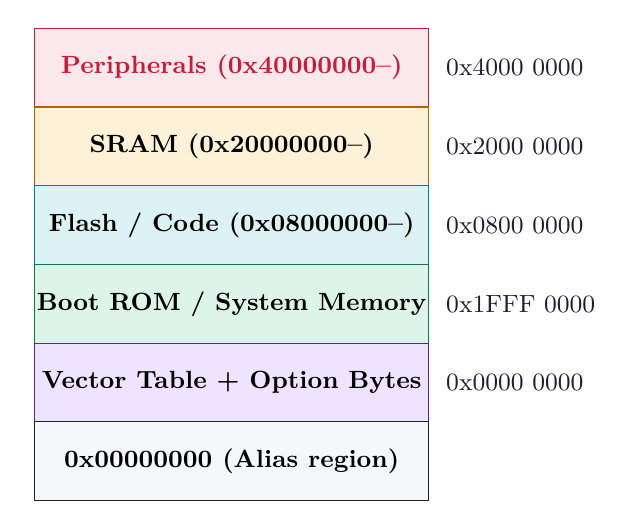
\begin{tikzpicture}[scale=1.0, every node/.style={font=\small}]
  % Memory blocks stacked vertically
  \draw[fill=hdrred, draw=myred] (0,5.0) rectangle (5,6.0)
    node[midway, font=\small\bfseries, color=myred] {Peripherals (0x40000000--)};
  \draw[fill=hdramber, draw=myamber] (0,4.0) rectangle (5,5.0)
    node[midway, font=\small\bfseries] {SRAM (0x20000000--)};
  \draw[fill=hdrteal, draw=myteal] (0,3.0) rectangle (5,4.0)
    node[midway, font=\small\bfseries] {Flash / Code (0x08000000--)};
  \draw[fill=hdrgreen, draw=mygreen] (0,2.0) rectangle (5,3.0)
    node[midway, font=\small\bfseries] {Boot ROM / System Memory};
  \draw[fill=hdrpurple, draw=mypurple] (0,1.0) rectangle (5,2.0)
    node[midway, font=\small\bfseries] {Vector Table + Option Bytes};
  \draw[fill=mygray, draw=mydark] (0,0.0) rectangle (5,1.0)
    node[midway, font=\small\bfseries] {0x00000000 (Alias region)};
  % Addresses
  \node[right, color=mydark] at (5.1, 5.5) {0x4000 0000};
  \node[right, color=mydark] at (5.1, 4.5) {0x2000 0000};
  \node[right, color=mydark] at (5.1, 3.5) {0x0800 0000};
  \node[right, color=mydark] at (5.1, 2.5) {0x1FFF 0000};
  \node[right, color=mydark] at (5.1, 1.5) {0x0000 0000};
\end{tikzpicture}
\end{tcolorbox}

% ===============================================================================
\section{Parallelism in Instruction Level}
% ===============================================================================

\begin{tcolorbox}[defbox, title={\textbf{Instruction-Level Parallelism (ILP)}}]
\textbf{Instruction-Level Parallelism (ILP)} is the ability of a processor to execute multiple instructions simultaneously, overlapping their execution stages using techniques such as \textbf{pipelining}, \textbf{superscalar execution}, and \textbf{VLIW} (Very Long Instruction Word).
\end{tcolorbox}

\subsection{Pipelining}

Pipelining divides instruction execution into \textbf{stages}, so that multiple instructions can be in different stages of execution simultaneously --- like an assembly line.

\begin{tcolorbox}[tikzbox, title={3-Stage Instruction Pipeline (ARM Cortex-M0)}]
\centering
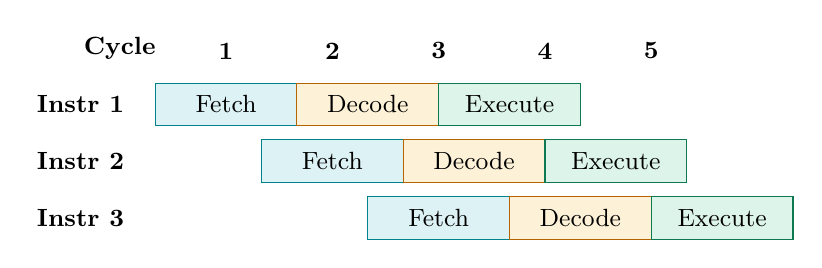
\begin{tikzpicture}[scale=0.9, every node/.style={font=\small}]
  % Stage labels
  \node[above] at (1.0, 3.2) {\textbf{Cycle}};
  \node[above] at (2.5, 3.2) {\textbf{1}};
  \node[above] at (4.0, 3.2) {\textbf{2}};
  \node[above] at (5.5, 3.2) {\textbf{3}};
  \node[above] at (7.0, 3.2) {\textbf{4}};
  \node[above] at (8.5, 3.2) {\textbf{5}};

  % Instruction 1
  \node[left] at (1.2, 2.7) {\textbf{Instr 1}};
  \draw[fill=hdrteal, draw=myteal] (1.5,2.4) rectangle (3.5,3.0) node[midway] {Fetch};
  \draw[fill=hdramber, draw=myamber] (3.5,2.4) rectangle (5.5,3.0) node[midway] {Decode};
  \draw[fill=hdrgreen, draw=mygreen] (5.5,2.4) rectangle (7.5,3.0) node[midway] {Execute};

  % Instruction 2
  \node[left] at (1.2, 1.9) {\textbf{Instr 2}};
  \draw[fill=hdrteal, draw=myteal] (3.0,1.6) rectangle (5.0,2.2) node[midway] {Fetch};
  \draw[fill=hdramber, draw=myamber] (5.0,1.6) rectangle (7.0,2.2) node[midway] {Decode};
  \draw[fill=hdrgreen, draw=mygreen] (7.0,1.6) rectangle (9.0,2.2) node[midway] {Execute};

  % Instruction 3
  \node[left] at (1.2, 1.1) {\textbf{Instr 3}};
  \draw[fill=hdrteal, draw=myteal] (4.5,0.8) rectangle (6.5,1.4) node[midway] {Fetch};
  \draw[fill=hdramber, draw=myamber] (6.5,0.8) rectangle (8.5,1.4) node[midway] {Decode};
  \draw[fill=hdrgreen, draw=mygreen] (8.5,0.8) rectangle (10.5,1.4) node[midway] {Execute};
\end{tikzpicture}
\end{tcolorbox}

\subsection{Pipeline Hazards}

\par\noindent
{\renewcommand{\arraystretch}{1.55}%
\begin{tabularx}{\linewidth}{|B{3.0cm}|Y|Y|}
\hline
\textbf{Hazard Type} & \textbf{Cause} & \textbf{Solution} \\
\hline
\textbf{Data Hazard} & Instruction depends on result of a previous instruction still in pipeline & Register forwarding (bypassing), stall/bubble insertion \\
\hline
\textbf{Control Hazard} & Branch instruction changes program flow before pipeline completes & Branch prediction, pipeline flush \\
\hline
\textbf{Structural Hazard} & Two instructions need same hardware resource simultaneously & Resource duplication, stall \\
\hline
\end{tabularx}}

% ===============================================================================
\section{Processor and Memory Selection}
% ===============================================================================

Selecting the right processor and memory for an embedded application requires balancing multiple constraints:

\begin{tcolorbox}[formulabox, title={\textbf{Processor Selection Criteria}}]
\begin{itemize}[leftmargin=*, itemsep=3pt]
  \item \textbf{Processing Speed:} Clock frequency (MHz) and MIPS (Million Instructions Per Second) rating.
  \item \textbf{Word Width:} 8-bit (simple, low-cost) vs.\ 16-bit vs.\ 32-bit (high performance).
  \item \textbf{On-chip Peripherals:} Required ADC channels, communication ports, timers.
  \item \textbf{Power Consumption:} Active current ($I_{DD}$), sleep current ($I_{standby}$) --- critical for battery-powered devices.
  \item \textbf{Cost:} Unit price must fit product BOM (Bill of Materials) budget.
  \item \textbf{Toolchain and Ecosystem:} Availability of compilers, debuggers, libraries, and community support.
  \item \textbf{Temperature Range:} Industrial ($-40^{\circ}$C to $+85^{\circ}$C), automotive ($-40^{\circ}$C to $+125^{\circ}$C).
\end{itemize}
\end{tcolorbox}

\subsection{Memory Selection Criteria}
\begin{itemize}[leftmargin=*, itemsep=3pt]
  \item \textbf{Volatile vs.\ Non-volatile:} Program code needs non-volatile (Flash); variables need volatile (SRAM).
  \item \textbf{Capacity:} Must accommodate program code, constants, variables, stack, and heap with margin.
  \item \textbf{Access Speed:} RAM access time must be compatible with processor clock (no wait states needed).
  \item \textbf{Endurance:} Flash has limited write cycles ($\sim$100,000 erase/write cycles) --- critical for OTA update designs.
  \item \textbf{Interface:} Parallel bus (faster) vs.\ serial (SPI/I2C Flash --- slower but fewer pins).
\end{itemize}

% ===============================================================================
% MANDATORY QUICK REVISION PAGE
% ===============================================================================
\newpage
\begin{center}
  {\large\bfseries\color{myred} Quick Revision --- Module 2}\\[3pt]
  {\small\color{mydark} Embedded Hardware: Processor \& Memory $|$ PE-EC703A}
\end{center}
\noindent{\color{myred}\rule{\linewidth}{1.2pt}}
\vspace{4pt}

\begin{tcolorbox}[formulabox, title={\textbf{Key Formulas at a Glance}}]
\renewcommand{\arraystretch}{1.3}
\begin{tabularx}{\linewidth}{B{4.5cm} X}
Machine Cycle Time (8051) & $t_{mc} = \displaystyle\frac{12}{f_{osc}}$ \quad (12 oscillator periods per machine cycle) \\[4pt]
Processing Speed & $\text{MIPS} = \displaystyle\frac{f_{clk}}{CPI \times 10^6}$ \quad (CPI = Cycles Per Instruction) \\[4pt]
Pipeline Speedup & $S = \displaystyle\frac{t_{no\text{-}pipeline}}{t_{pipeline}} \approx N$ \quad ($N$ = number of stages, ideal) \\[4pt]
Memory Address Space & $\text{Addressable locations} = 2^n$ \quad ($n$ = address bus width in bits)
\end{tabularx}
\end{tcolorbox}

\begin{tcolorbox}[defbox, title={\textbf{One-Line Definitions}}]
\begin{itemize}[leftmargin=*, itemsep=2.5pt, topsep=0pt]
  \item \textbf{8051:} An 8-bit Harvard-architecture microcontroller with 4 KB ROM, 128 B RAM, 4 I/O ports, and 2 timers.
  \item \textbf{ARM:} Advanced RISC Machine; 32-bit low-power RISC processor widely used in embedded and mobile devices.
  \item \textbf{RISC:} Reduced Instruction Set Computer --- few, simple, fixed-length instructions; high clock rate.
  \item \textbf{Harvard Architecture:} Separate buses for program memory and data memory allowing simultaneous access.
  \item \textbf{Von Neumann:} Single shared bus for instructions and data; simpler but slower.
  \item \textbf{Pipeline:} Technique to overlap execution of multiple instructions by dividing into fetch-decode-execute stages.
  \item \textbf{ILP:} Instruction-Level Parallelism --- executing multiple instructions in the same clock cycle.
  \item \textbf{Flash Memory:} Non-volatile, electrically erasable memory used to store program code in MCUs.
  \item \textbf{SRAM:} Static RAM --- volatile, fast, no refresh; used for data memory and stack in MCUs.
  \item \textbf{SFR:} Special Function Register in 8051 (addresses 80H--FFH) controlling timers, serial port, I/O, interrupts.
  \item \textbf{Thumb Instruction Set:} 16-bit compressed ARM instruction set reducing code size by $\sim$30\%.
  \item \textbf{NVIC:} Nested Vectored Interrupt Controller in ARM; handles priority-based, low-latency interrupts.
\end{itemize}
\end{tcolorbox}

\begin{tcolorbox}[exambox, title={\textbf{Frequently Asked / Viva Questions}}]
\begin{enumerate}[topsep=0pt, label=\textbf{Q\arabic*.}, itemsep=5pt]
  \item \Q{What is the architecture of the 8051 microcontroller?}
    The 8051 is an 8-bit Harvard-architecture MCU with a 4 KB ROM (program), 128 bytes RAM (data), four 8-bit I/O ports, two 16-bit timers, one UART serial port, and five interrupt sources. One machine cycle = 12 oscillator clock cycles.
  \item \Q{What is the difference between Harvard and Von Neumann architecture?}
    Harvard uses separate buses for program and data memory, enabling simultaneous fetch and data access (faster). Von Neumann uses a single bus for both (simpler but has bottleneck). 8051 and ARM MCUs use Harvard; x86 PCs use Von Neumann.
  \item \Q{What is pipelining? What is its advantage?}
    Pipelining divides instruction execution into stages (Fetch, Decode, Execute) and processes multiple instructions concurrently in different stages. Advantage: Increases throughput (instructions completed per clock cycle) without increasing clock frequency.
  \item \Q{Name the three types of pipeline hazards.}
    \begin{itemize}[leftmargin=*, itemsep=1pt, topsep=2pt]
      \item \textbf{Data Hazard:} Dependency between instructions (solved by forwarding/stall).
      \item \textbf{Control Hazard:} Branch instructions disrupting pipeline flow (solved by branch prediction).
      \item \textbf{Structural Hazard:} Two instructions compete for same hardware resource.
    \end{itemize}
  \item \Q{Why is ARM preferred over 8051 for modern embedded systems?}
    ARM (Cortex-M) offers 32-bit data width, higher clock speeds (up to 168 MHz), a pipelined RISC core, Thumb instruction set for code efficiency, built-in NVIC, optional FPU/DSP, and ultra-low power modes. 8051 is only 8-bit and runs at 12 MHz.
  \item \Q{What is the Thumb instruction set in ARM?}
    Thumb is a 16-bit compressed version of the 32-bit ARM instruction set. It reduces code size by $\sim$30\% while retaining most of the performance, making it ideal for memory-constrained embedded systems.
  \item \Q{What are Special Function Registers (SFRs) in 8051?}
    SFRs are memory-mapped registers (addresses 80H--FFH) that control the MCU's internal peripherals such as ports (P0--P3), timers (TCON, TMOD), serial port (SCON, SBUF), interrupt control (IE, IP), and the stack pointer (SP).
  \item \Q{What is the difference between Flash memory and EEPROM?}
    Flash memory is erased in large \textbf{blocks/pages} and is much faster and higher-density --- used for program code storage. EEPROM is erased byte-by-byte (or word-by-word), has fewer erase cycles, but allows fine-grained updates --- used for configuration data.
  \item \Q{What factors are considered in processor selection for an embedded system?}
    Processing speed (MIPS), word width (8/16/32-bit), on-chip peripheral set, power consumption, operating temperature range, unit cost, and availability of compilers, development tools, and community support.
  \item \Q{What is memory-mapped I/O?}
    In memory-mapped I/O, peripheral registers (I/O ports, timers, UART) are assigned addresses in the same address space as RAM. The processor accesses them using regular memory read/write instructions --- no separate I/O instructions needed (used in ARM Cortex-M).
  \item \Q{What is the significance of the barrel shifter in ARM?}
    The barrel shifter in ARM's ALU allows any data-processing instruction to optionally shift or rotate one of its source operands by any amount \textbf{in the same clock cycle} as the main operation --- effectively providing free shift operations.
  \item \Q{What is MIPS and how is it calculated?}
    MIPS (Million Instructions Per Second) measures processor performance. $\text{MIPS} = f_{clk} / (CPI \times 10^6)$ where CPI is Cycles Per Instruction. For 8051 at 12 MHz with CPI = 12: MIPS $= 12/(12) = 1$ MIPS.
\end{enumerate}
\end{tcolorbox}

\begin{tcolorbox}[tikzbox, title={8051 vs.\ ARM Cortex-M --- At a Glance}]
\par\noindent
{\renewcommand{\arraystretch}{1.55}%
\begin{tabularx}{\linewidth}{|B{2.8cm}|Y|Y|}
\hline
\textbf{Parameter} & \textbf{8051} & \textbf{ARM Cortex-M4} \\
\hline
\textbf{Data Width} & 8-bit & 32-bit \\
\hline
\textbf{Max Clock} & 12 MHz (standard) & 168 MHz \\
\hline
\textbf{Architecture} & Harvard, CISC-like & Harvard, RISC \\
\hline
\textbf{Pipeline} & None & 6-stage \\
\hline
\textbf{On-chip Flash} & 4 KB (original) & Up to 2 MB \\
\hline
\textbf{On-chip SRAM} & 128 bytes & Up to 256 KB \\
\hline
\textbf{FPU} & No & Yes (single precision) \\
\hline
\textbf{Interrupts} & 5 sources & Up to 240 (NVIC) \\
\hline
\end{tabularx}}
\end{tcolorbox}

\end{document}
